% !TeX root = ../main.tex

\chapter{Resultados}

\section{Descripción de Datos Filtrados}

    Para garantizar la robustez estadística de los parámetros estructurales 
    derivados, la muestra inicial de 100 cúmulos fue sometida a un proceso de 
    depuración de datos anómalos. Este procedimiento de selección se implementó 
    aplicando el método del rango intercuartílico (IQR) de forma bivariada sobre 
    los valores del radio de núcleo tridimensional ($r_c$) y la masa total del 
    cúmulo ($M_{\text{total}}$). La efectividad de este criterio estadístico es 
    evidente al analizar la distribución de las escalas espaciales internas, 
    donde los sistemas excluidos presentaban extensiones extremas; el filtrado 
    permitió consolidar una muestra refinada cuyos radios de núcleo se 
    concentran predominantemente en un régimen físicamente cohesivo, por debajo 
    de los $13\text{ pc}$.

    Al evaluar la bondad de ajuste de los perfiles de densidad espacial 
    tridimensional mediante el estadístico $\chi^2$, se evidencia una clara 
    estratificación en la confiabilidad de los modelos analíticos en función de 
    la masa del cúmulo. En el plano de $\log(\chi^2)$ respecto a 
    $\log(M_{\text{total}}/\text{M}_\odot)$, los cúmulos retenidos tras el 
    filtro IQR abarcan un rango de masas totales comprendido mayoritariamente 
    entre $10^{2.8} \text{ M}_\odot$ y $10^{4.0} \text{ M}_\odot$. Para este 
    subconjunto robusto, el logaritmo del estadístico de prueba se mantiene 
    consistentemente acotado, distribuyéndose en un intervalo aproximado de 
    $-0.2$ a $0.8$. Por el contrario, los sistemas catalogados como atípicos y 
    excluidos del análisis subsiguiente tienden a segregar hacia el régimen de 
    masas más elevadas, superando los $10^{4.0} \text{ M}_\odot$, y exhiben 
    simultáneamente dispersiones mayores en la bondad de ajuste, con valores de 
    $\log(\chi^2)$ que superan sistemáticamente el umbral de $0.4$ y alcanzan 
    picos por encima de $1.0$. Esta divergencia paramétrica indica que el modelo 
    clásico de King resulta notablemente menos representativo, o presenta 
    mayores discrepancias en la minimización de los residuales, para las 
    agrupaciones estelares más masivas de la muestra, validando de manera 
    independiente la idoneidad del corte estadístico implementado.
    
    \begin{figure}[htbp]
        \centering
        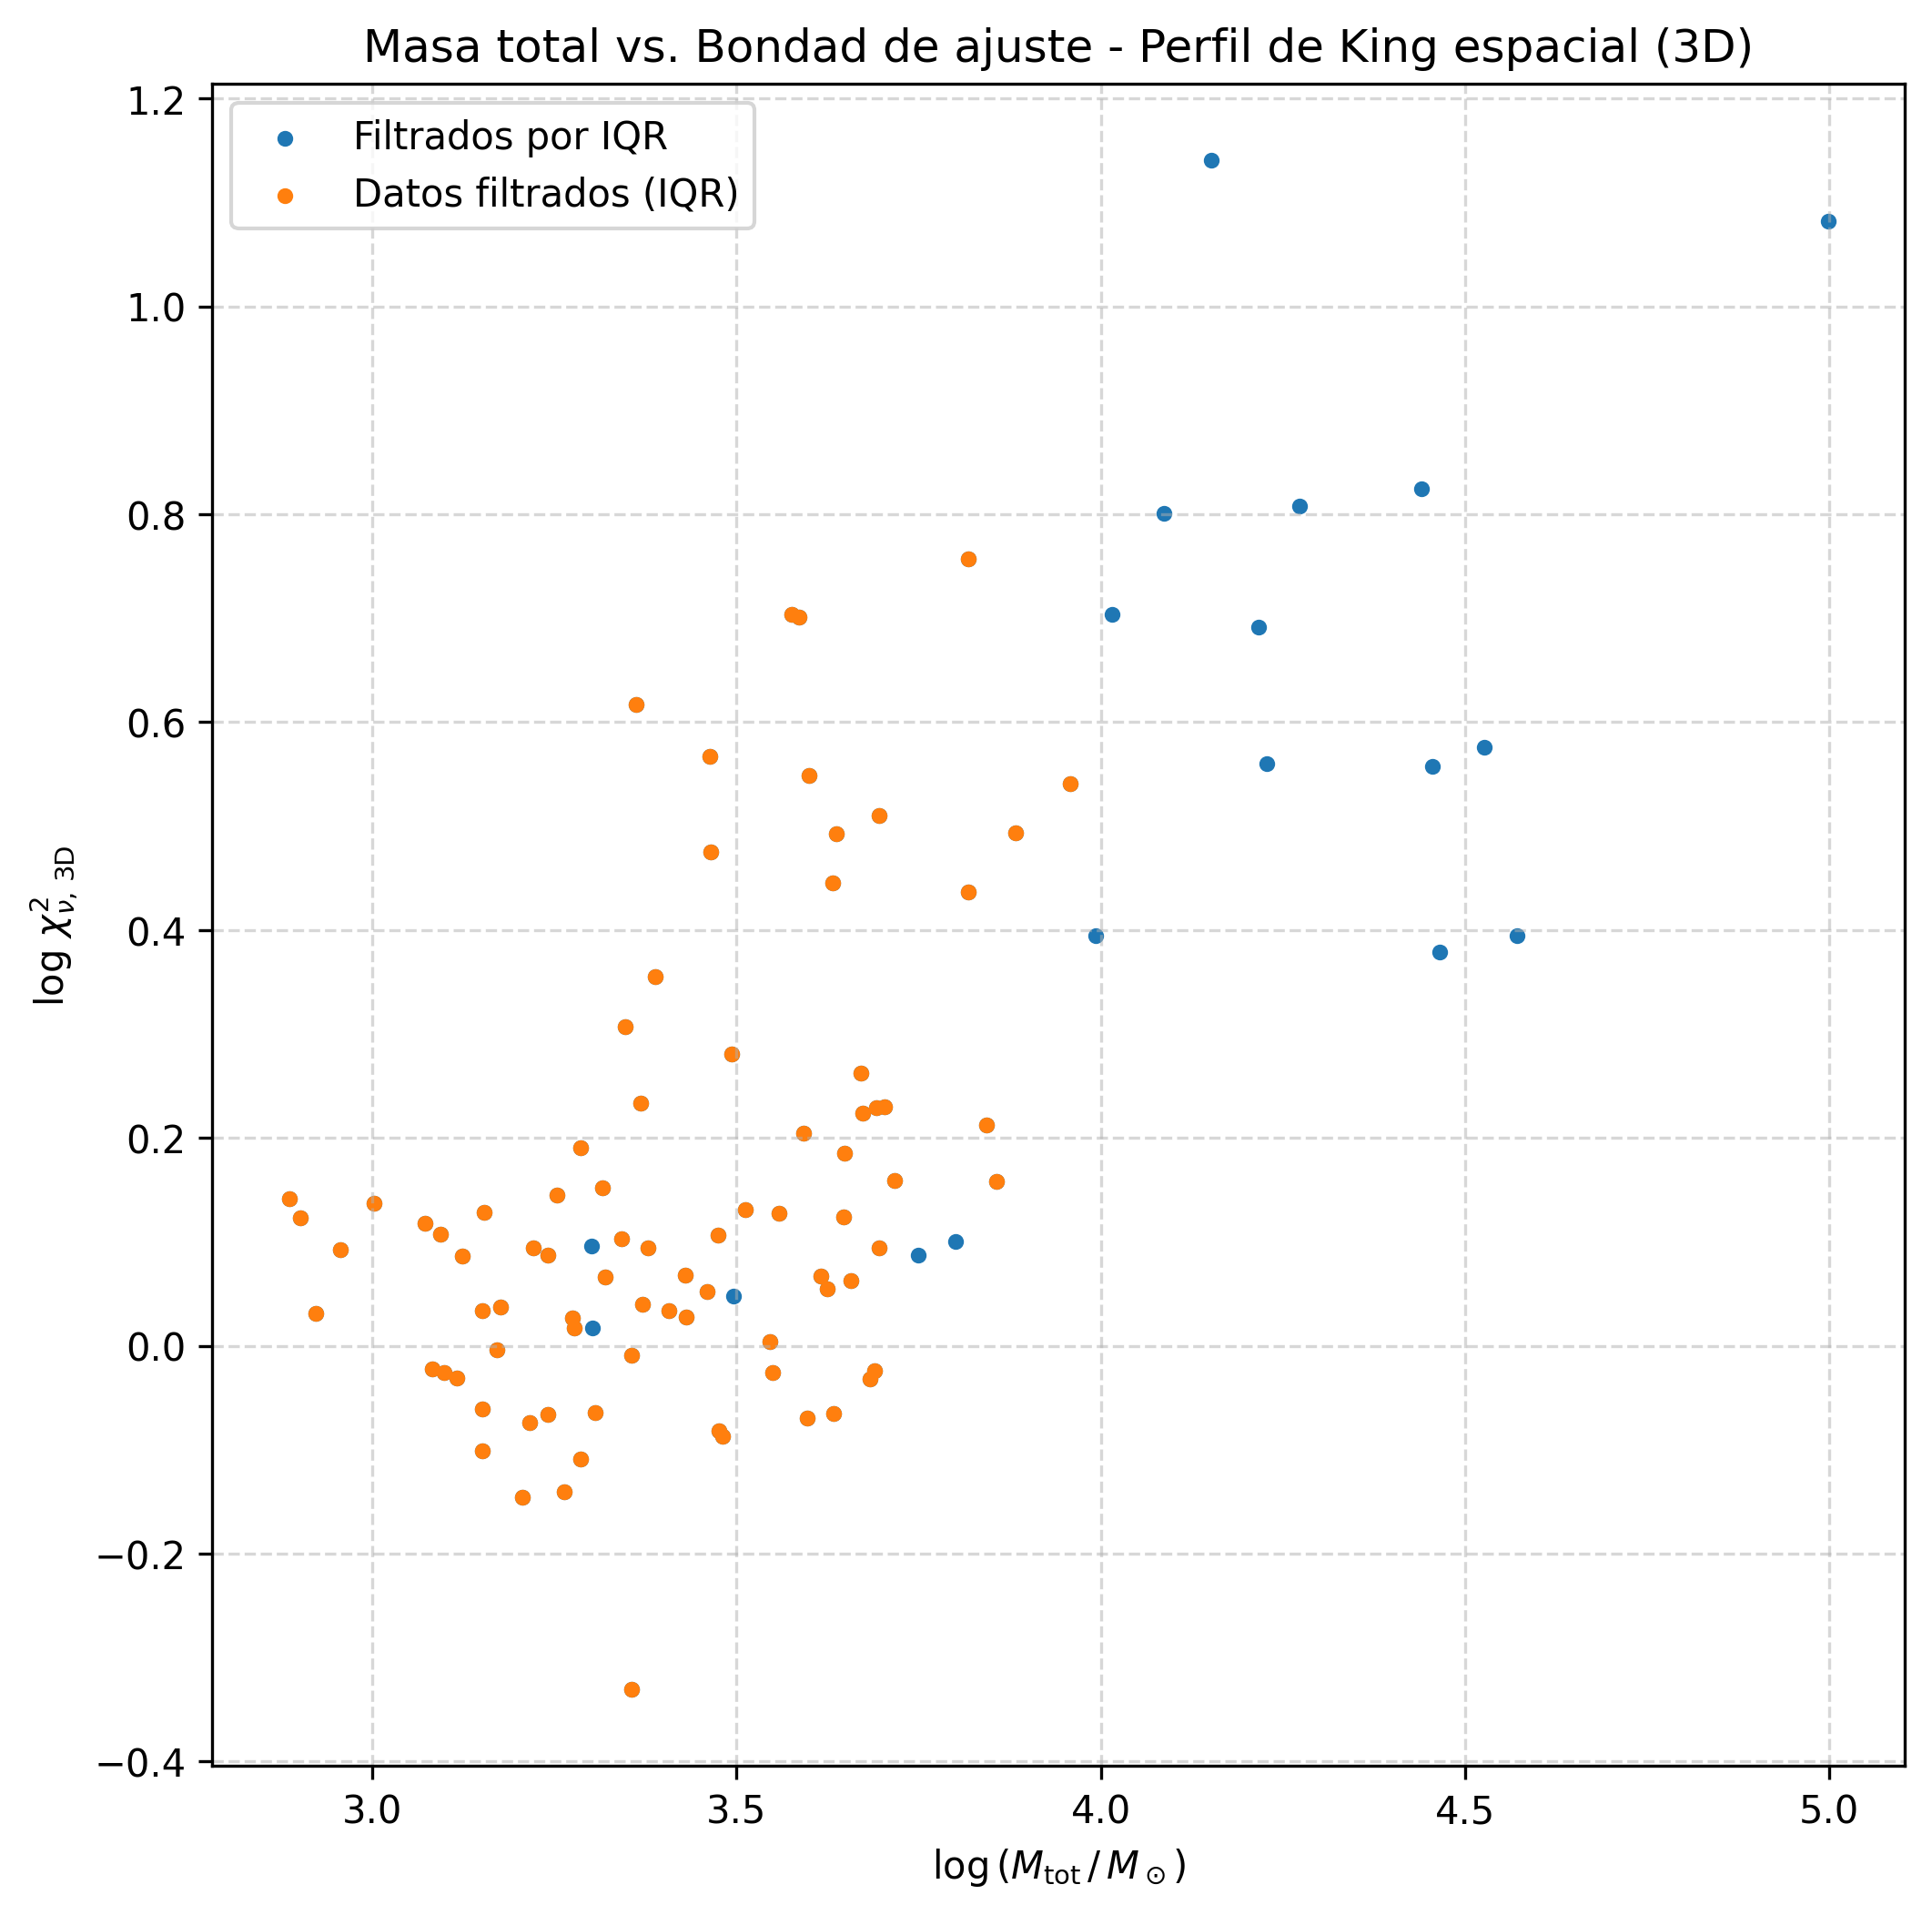
\includegraphics[width=0.8\textwidth]{imagenes/masa_vs_chi2_king3d.png}
        \caption{
            Relación entre la masa total de los cúmulos, 
            $\log(M_{\text{tot}}/\text{M}_\odot)$, y la bondad de ajuste de sus 
            respectivos perfiles de densidad espacial de King, evaluada mediante 
            el estadístico $\chi^2$ reducido ($\log \chi^2_{\nu,\text{3D}}$). 
            Los puntos en color naranja identifican la muestra consolidada de 
            cúmulos tras aplicar el filtro IQR. En contraste, los puntos azules 
            representan los sistemas estadísticamente atípicos que fueron 
            excluidos del análisis. Se evidencia una tendencia en la que las 
            agrupaciones estelares de mayor masa exhiben desviaciones más 
            pronunciadas respecto al modelo analítico.
            }
        \label{fig:masa_vs_chi2_3d}
    \end{figure}